% !TEX encoding = UTF-8 Unicode
% !TEX program = pdflatex
% !TEX spellcheck = en_US


% In order to correctly compile this document,
% execute the following commands:
% 1. pdflatex
% 2. pdflatex
% 3. pdflatex



\documentclass[amsthm,ebook]{saparticle}

% IF YOU USE PDFLATEX
\usepackage[utf8x]{inputenc}
% if you write in english and in greek
\usepackage{ucs}
\usepackage[greek,english]{babel}
\languageattribute{greek}{polutoniko}

\usepackage{teubner}
% IF YOU USE XELATEX
%\usepackage{polyglossia}
% if you write in italian
%\setmainlanguage{italian}
% If you want put some ancient greek:
%\setotherlanguage[variant=polytonic]{greek}
%\newfontfamily{\greekfont}[Ligatures=TeX]{Palatino Linotype}

% dummy text (remove in a normal thesis)
% remove if not necessary
\usepackage{siunitx}
%Natbib for bibliography management
\usepackage[authoryear]{natbib}
% custom commands
\newcommand{\bs}{\textbackslash}

%%%%%%%%
%TITLE:%
%%%%%%%%
\title{Tradition and progress. The Roman World in the Digital Age - seen through Inscriptions}
%\author[]{Werner Eck\corref{first}}
\author[koe]{Werner Eck\corref{first}}
\address[koe]{Universität zu Kölln} 
\cortext[first]{Corresponding author. Email: Werner.Eck@uni-koeln.de}
\begin{document}
\maketitle
%\begin{abstract}
%\end{abstract}

Epigraphy has caught up with the digital age. If this point needs to be proven, 
this very conference speaks for itself.  Its celebration in Rome does not happen 
by chance. Indeed, the first real attempt to create a collective compilation and 
presentation of all the Latin (and Greek) inscriptions in a single database or 
as a connection of the existing databases was made here in Rome in 1997 through 
Silvio Panciera during the 11\textsuperscript{th} International Congress of Greek 
and Latin Epigraphy\footnote{See S. Panciera, Informatica, in: idem, Epigrafi, epigrafia, epigrafisti, vol. 2, Rome 2006, 1913ff. – I would like to thank Aitor Blanco Perez for the translation of the paper.}. His fundamental initiative set in motion a process, which 
step by step will lead to a complete database. Very important steps in this direction 
have been made in the meantime and the development is progressing with particular 
emphasis at the Sapienza thanks to the collaboration between traditional epigraphists 
such as Silvia Orlandi and IT-people, who are affiliated to the Centro Linceo Beniamino 
Segre. These two and all the other partners in many European countries have to 
be thanked for these present steps and we wish them both courage and success in 
the following phase. 

Whoever is dealing with inscriptions, at least since the 16\textsuperscript{th} 
century, has to deal with a continuously growing mass phenomenon. One of the reasons, 
which instigated Mommsen to establish the \textit{CIL}, was the amount of epigraphic 
texts, which were known at that time but had not been collected in one single place 
but were, instead, spread in countless manuscripts and publications. Even when 
one looks into a representative selection such as the \textit{Inscriptiones Latinae 
Selectae }by Hermann Dessau – completed in 1916 – there are more than 9500 
texts. Since the time of Mommsen and Dessau, however, the number of epigraphic 
documents has increased to a size previously unknown. On the website of EAGLE one 
can read of more than 1.5 million items, currently scattered across 25 EU countries 
as well as the east and south Mediterranean, which should be collected in the EAGLE 
database. In order to illustrate this growth in a more accessible way, let me refer 
to the following example. Since the conclusion of the first edition of \textit{CIL 
II}, namely with the supplement in 1892, the number of inscriptions from the Iberian 
Peninsula has tripled. For some types of inscriptions, the increase is even bigger. 
When Herbert Nesselhauf collected all the military diplomata in 1935, he could 
put together a total of 187 documents in \textit{CIL XVI. }Today, we know more 
than 1100 such texts, i.e. an increase of 7 times. Not in all regions of the early 
Roman Empire and for all types of inscriptions is the increase as dramatic as in 
the aforementioned examples. Even so, a doubling can be identified in many Roman 
places. Just to mention some examples: in Sarmizegetusa, the first Roman colony 
following the conquest of Dacia, around 330 inscriptions were collected in the 
different volumes of \textit{CIL III.} Since then, more than the same number of 
new texts has appeared, perhaps around 400\footnote{According to information by Ioan Piso}. The growth is almost always dramatic 
when intensive excavations lead to a massive increase in the amount of inscriptions 
available, as somehow happens in the cases of Sagalassos or Perge in Pamphylia\footnote{In Sagalassos almost all the new inscriptions are in Greek}. 
Perge provided only 4 Latin inscriptions for the \textit{CIL III} and today there 
are at least 42\footnote{See the Clauss-Slaby database}. Even more dramatic is the growth in Caesarea Maritima. In \textit{CIL 
}there were only 3 Latin inscriptions known from the capital of the province of 
Judea, while now we have in the Corpus Inscriptionum Iudaeae/Palaestinae more than 
270 Latin documents\footnote{W. Eck, Comprendere contesti: Il nuovo multilingue Corpus Inscriptionum Iudaeae / Palaestinae, in: Rationes Rerum 1, 2013, 17 ff.}.   

Each of us is familiar with this massive increase in epigraphic monuments and we 
are reminded of this every year by the always more extensive volumes of \textit{AE} and \textit{SEG}. Even if it is impossible to provide an exact number of all the 
Latin inscriptions, one can still take as a starting point the fact that there 
are approximately 500.000 texts available for our work, including the so-called 
\textit{instrumentum domesticum}. There are more than 495.000 inscriptions in the 
Database Clauss-Slaby. Around 72.000 we can find in the Heidelberg Database and 
around the same number in the Epigraphic Database of Rome, from which the Project 
EAGLE emerged, not to mention other participants as, among others, \textit{Hispania 
Epigraphica }or the Bari Epigraphic Database \footnote{See the individual databases}. With regard to the Greek inscriptions, 
it is much more difficult to give an approximate number because their digital record 
is not as advanced as in the case of the Latin inscriptions. As for inscriptions 
in other languages – such as Punic, Hebrew-Aramaic, Demotic or Nabatean – let 
me exclude them from this discussion, even though they are just as part of the 
epigraphic tradition of the Greek and Roman antiquity as Latin and Greek inscriptions 
– we should not forget this very important fact\footnote{\label{fn:7}At the 14. International Congress of Greek and Latin Epigraphy there was a special section for this phenomenon: W. Eck, Ph. Hyse, J. Price, St. J. Seidlmayer, I.-X. Adiego, in: ÖFFENTLICHKEIT – MONUMENT – TEXT. XIV Congressus Internationalis Epigraphiae Graecae et Latinae Akten, hg. W. Eck - P. Funke, Berlin 2014, 159 ff}. Our work as historians or philologists 
is based on all those texts. But, the bigger the number of documents providing 
information is, the more difficult it becomes to find all texts. Even more difficult 
is to collect selectively those texts related to the topic on which one wants to 
work. And yet, the complete collection is crucial for the scientific result.

Let's go back only two or maybe three decades, a time which many of you in this 
room have vividly gone through. In that time it was clear, what we had to do, when 
we wanted to explore a topic on the basis of epigraphic evidence. We were to search 
– sometimes in countless volumes of inscriptions and partly supported through 
more or less detailed indexes. Depending on the type of subject on which we were 
working, these indexes were not always perfect tools to find the material. Very 
often they could not even be such perfect tools, since many phenomena are not accessible 
through precise termini in the epigraphic material, but rather through the entire 
content of the text. I am sure that you all have your own experiences. When I worked 
on the administration of Italy in the high Roman Empire, the indices were helpful 
but not sufficient. I had to go through each and every of the epigraphic corpora, 
which means that at least the inscriptions had to be read. In total, the look through 
all the necessary volumes took me almost two years. 

Is that different today because there are numerous databases available? At least 
with regard to the Latin inscriptions almost all of them are collected, although 
with very different individual information. With few clicks, we can find an answer 
for many questions in few seconds – sometimes one has to wait a bit longer, since 
the server does not work properly or some other problems exist. Indeed, as an already 
deceased colleague once told me long before the digital period in 1973: \textit{Pazienza} 
is the greatest virtue of the epigraphist. Today we are ready to forget this virtue 
thanks to our computers. At any rate, most of the relevant material available in 
databases appears quickly on the screen. It is not necessary to give examples. 
And yet, something which we all know: it is by no means guaranteed that we have 
found absolutely all the relevant material which exists; the reason for these gaps 
are inter alia, that not a small part of our epigraphic testimonies survives only 
as fragments and can be restored in different ways. For example, if we would try 
to find all the \textit{quaestores }of the province of Achaea in the imperial age, 
we would not find the following fragmentary inscription from Corinth, the capital 
of the province, because the text has read as follows\footnote{\emph{CIL III} 537}: 

\begin{quote}

{\it Q(uinto) Vili[o --] / Titia[no] / Quadra[to --] / IIIIvir(o) vi[ar(um) cur(andarum), trib(uno)] / la\mqs{t}icl(avio) \mqs{le}g(ionis) [--, \textbf{leg(ato) prov(inciae)] / Ach(aiae)}, ob ius[titiam et fidem,] / quam circa [universam] / Achaia[m exhibuit,] / qu\mqs{a}m pro pr(aetore) [administravit.] / \mqs{M}(arcus) An\mqs{to}nius M(arci) [f(ilius)] / Nigrinus [--].}
\end{quote}


Our search in a database would have recorded a proconsular legate of Achaea whose 
function in the inscription is nevertheless restored. The restoration of the position 
of provincial legate is not impossible, but it is also not very likely. The restoration 
of the office of quaestor:\textit{ [-- quaest(ori) prov(inciae)] / Ach(aiae) }instead 
of \textit{[-- leg(ato) prov(inciae)] / Ach(aiae) }fits in the lacuna much better\footnote{In the database Clauss-Slaby there are around 68 examples in Latin inscriptions, in the database of the Packard Institute on can find 10 more in Greek texts.}. 
For a young senator who had completed an office of the \textit{vigintiviri }and 
then a tribunate in the legion, the \textit{quaestura }should actually follow in 
a normal career and not the position of a proconsular legate under a proconsul. 
Of course, we know that exceptionally young senators already before the \textit{quaestura 
}were acting as legates of a proconsul in his province. In total, there are only 
four of such cases. By contrast, much more senators state in their inscriptions 
that they have held the office of provincial \textit{quaestor} as\textit{ pro praetore}. 
The \textit{pro pr(aetore) }preserved in the inscription could therefore refer 
to the \textit{quaestura}. As the \textit{quaestura }normally follows the\textit{ 
}viginvirate and the legionary tribunate, this rule should automatically be observed 
in a fragmentary career\footnote{See now the new reconstruction of the inscription by W. Eck, Quaestor, nicht legatus provinciae Achaiae. Zu einer Inschrift des Q. Vilius Quadratus aus Korinth, (in preparation).}. This kind of result is not achieved through an inquiry 
into a database but through a constructive consideration on the basis of personal 
experience. Such knowledge will remain also the basis of our discipline in the 
future. Databases complement our knowledge but they cannot replace it. This can't 
be their business. 

Inscriptions are in the first place texts which contain certain evidence as such. 
But inscriptions do not only consist of text, although this may commonly seem to 
be the case in the literature. In German, one speaks of ``\textit{Inschriften 
errichten}'' and in Italy one can say: \textit{una iscrizione eretta}\footnote{It seems not necessary to give examples for this type of formulation; they are abundant.}. In the Prosopographia 
Imperii Romani,\textit{ }the expression \textit{titulum ponere }was long in use 
and applied to inscriptions of all kinds. With these expressions, it was not clear, 
what specific function was connected with an epigraphic text and the support on 
which the inscription appears. Nonetheless, the support already contains its own 
message and that was, on many occasions, the primary message for the Greek and 
Roman public\footnote{\label{fn:12}Cf. now W. Eck, Wie ehrt man Mitglieder der staatlich-städtischen Elite? Inschriftenbasen unerkannter Reiterdenkmäler, Kolloquium Kassel März 2015, hg. K. Ruffing – H. Schneider (in print)}. In order to understand what an inscription can today convey as evidence, 
it is fundamental to include the \textbf{monument }with which the inscription was 
connected. This can be an altar, an architrave of a temple, a mausoleum or, for 
instance, the base for a statue, which is explained by the inscription. In enquiring 
about the content of inscriptions, we muss decisively take into consideration the 
function that inscription and monument shared in the Graeco-Roman world. 

However, when one looks for the function of an inscription in a database, the difficulties 
begin – if I were to speak about my own experiences. On many occasions, this 
function is not found, if one enquires about what is directly conveyed in the inscription, 
because this exact function is commonly not mentioned in the epigraphic text. This 
is not surprising. To mention the function was not particularly necessary because 
the ancient observer completely saw, on what an inscription was written. Given 
that today this context is mostly not preserved, we must infer it from the support 
whose form and particular details are connected with it. This necessity has meanwhile 
become almost common knowledge – in contrast with Mommsen's time\footnote{W. Eck, Mommsen e il metodo epigrafico, in: Concordia e la X Regio. Giornate di Studio in onore di Dario Bertolini, Atti del Convegno Portogruaro 22-23 ottobre 1994, Padova 1995, 107 ff.}. On the EAGLE 
website, this is specifically taken into account with the option \textit{advanced 
search, }in which it is possible to browse the database according to object type. 
With this option, one can find the categories, for example, of \textit{statue, 
statue base, statue base shaft or plinth}. Hence it is already possible to obtain 
a result with a high degree of differentiation, if one browses selectively. However, 
not all the different categories of statues are grasped with these search terms. 
Just to mention an example: \textit{bigae }or \textit{quadrigae, }which were erected 
to honour a person, can only be found if these terms would also appear in the inscription. 
But in the epigraphic text the object is directly mentioned only in a limited number 
of cases. The ancient observer saw the object which did not need any additional 
reference. For us, on the other hand, the specific types of statues are generally 
recognisable only if we include the support of the inscription in the analysis. 
The original statues are almost always lost or, at least, not connected with the 
inscription. Enquiring about the types of statues is not a child's play. For the 
most part, they rather say fundamental things for both the honoured and the honouring 
individuals. 

One example from Volsinii (modern Bolsena) can illustrate this\footnote{AE 1980, 426.}. It is an honorific 
monument set up to commemorate a senator of the Hadrianic-Antonine age. The surviving 
fragmentary \textit{titulus honorarius }records his names: Pompeius Vopiscus C. 
Arruntius Catellius Celer Allius Sabinus, followed by his \textit{cursus }and, 
finally, the city of Carthage as dedicator. The text, however, does not specify 
in which figurative way the senator was presented to the audience of ancient Volsinii. 
This is also not attempted in the epigraphic database of Rome; there it is only 
said (as in the Epigraphischen Datenbank Heidelberg) that the text is to be read 
on a base\footnote{EDR077846 = HD005099 (M.G. Schmidt).}. While this is correct, the plain term ``base'' does not allow to recognise 
the most important element, namely with what type of honour had the city of Carthage 
honoured the senator coming from Volsinii. The particular quality of the honour 
is, nevertheless, revealed by the size and shape of the inscribed plaque. The plaque 
is 76.5 cm high and 1.90 m wide\footnote{P. Gros, MEFRA 92, 1980, 977 ff.}. The monument was so wide that a normal statue 
could not have stood on it; this would have appeared completely out of place. Given 
the width of the inscribed slab, it is to be inferred that a \textit{biga }or perhaps 
even a \textit{quadriga} was set up for the senator\textit{.} He should therefore 
have completed an action beyond his official duty on behalf of Carthage for which 
the city decided to recognise his activity in this lavish way and to send ambassadors 
to Volsinii to erect the monument.      

A similar case can be inferred for Larcius Priscus, a legate of the \textit{legio 
III Augusta}\footnote{\emph{CIL VIII} 17891 = Dessau 1055.}. The city of Thamugadi honoured him in a similar way to that of Carthago 
for the senator in Volsinii. On the forum of the colony founded by Trajan, not 
a normal honorary statue not even an equestrian statue – as previously suspected\footnote{\label{note:18}J. Bergemann, Römische Reiterstatuen. Ehrendenkmäler im öffentlichen Bereich, Mainz 1990, 147 Nr. E 90:  ``equestrian statue''.} 
– was set up but rather a \textit{biga }on which the statue of Larcius Priscus 
was presented to the citizens of Timgad\footnote{The inscription is 188 cm wide, much more than necessary for an equestrian statue.}. But in EAGLE one finds the note: 

Type of object: unbestimmt = undefined (= EDH)\footnote{EDH031159 (B. Gräf).}. 

But one can see the type of the object on the photo, published by Zimmer in 1989\footnote{G. Wesch-Klein, Katalog der Inschriften, in: G. Zimmer, Locus datus decreto decurionum. Zur Statuenaufstellung zweier Forumsanlagen im römischen Africa, München 1989, 71 Nr. T 4.}. 
More examples of this kind could be given. In my opinion, an important consequence 
is therefore clear. If databases were to fulfil their function completely, then 
it would be not only useful but rather very necessary to record an indication of 
the concrete form of the honorific monument in such cases. Otherwise, a crucial 
part of the potential information would be lost.  

Of course such a degree of precision is not always possible, but very likely when 
– as shown by the two previous examples – the form of the support provides 
evidence beyond the text of the inscription that can be searched in the database. 
This happens for example in many inscriptions which in antiquity were to be seen 
under \textit{statuae equestres}. Sometimes this form of honour is recorded in 
the text of the inscription itself. In the database Clauss, there are around 45 
records if one looks for \textit{statuae equestres }or \textit{statuam equestrem},\textit{ 
}in the database EAGLE around 27. That EAGLE shows fewer cases is naturally due 
to the fact that this database is still under construction. Either with 45 or 22 
inscriptions, this only records in any case a minority of the texts which were 
once to be read under such \textit{statuae equestres}. In the monograph on equestrian 
statues written by Johannes Bergemann in 1990, 128 inscriptions are collected, 
which were once connected with an equestrian statue according to the investigations 
of the author \footnote{See n. \ref{note:18}.}. Besides the statues directly referred to as such in the text, there 
are also those containing other hints which allow us to recognise that the honoured 
person was once presented on a horse. 



Some examples should illustrate which equestrian statues cannot be recognised as 
such without these extra hints. In the colonia Aelia Capitolina, modern Jerusalem, 
an equestrian statue was erected for Antoninus Pius through the council of decurions, 
apparently straight after his accession in the year 138/9. In the text of the honorific 
inscription, the type of statue is not mentioned but it can be inferred from the 
size of the inscription\footnote{Corpus Inscriptionum Iudaeae/Palaestinae I 2, 718.}. Therefore, it must be registered as an equestrian statue 
in a database. The same applies to the honours bestowed in Lepcis Magna upon the 
governor of the late-antique province Tripolitana, Flavius Nepotianus. In the inscription 
itself, it is only spoken of a \textit{statua marmorea} that should memorialise 
the services of the magistrate\footnote{IRT 565.}. However, the base enables to recognise that a \textit{statua 
equestris }once stood there because this base is 170 cm deep\footnote{Bergemann (n. \ref{note:18}) no. 83. Cf. the inscription for the flamen provinciae Pompeius Cerealis Salvianus in Lepcis Magna: the basis is 70 cm high, but 160 cm deep (IRT 602).}. 

\begin{figure}[!bp]
\centering
 \includegraphics[scale=0.5]{images/fig01ReiterstatueZeichnung.pdf}
\caption{Equestrian statue: drawing}
\label{fig:1}
\end{figure}

\begin{figure}[!bp]
\centering
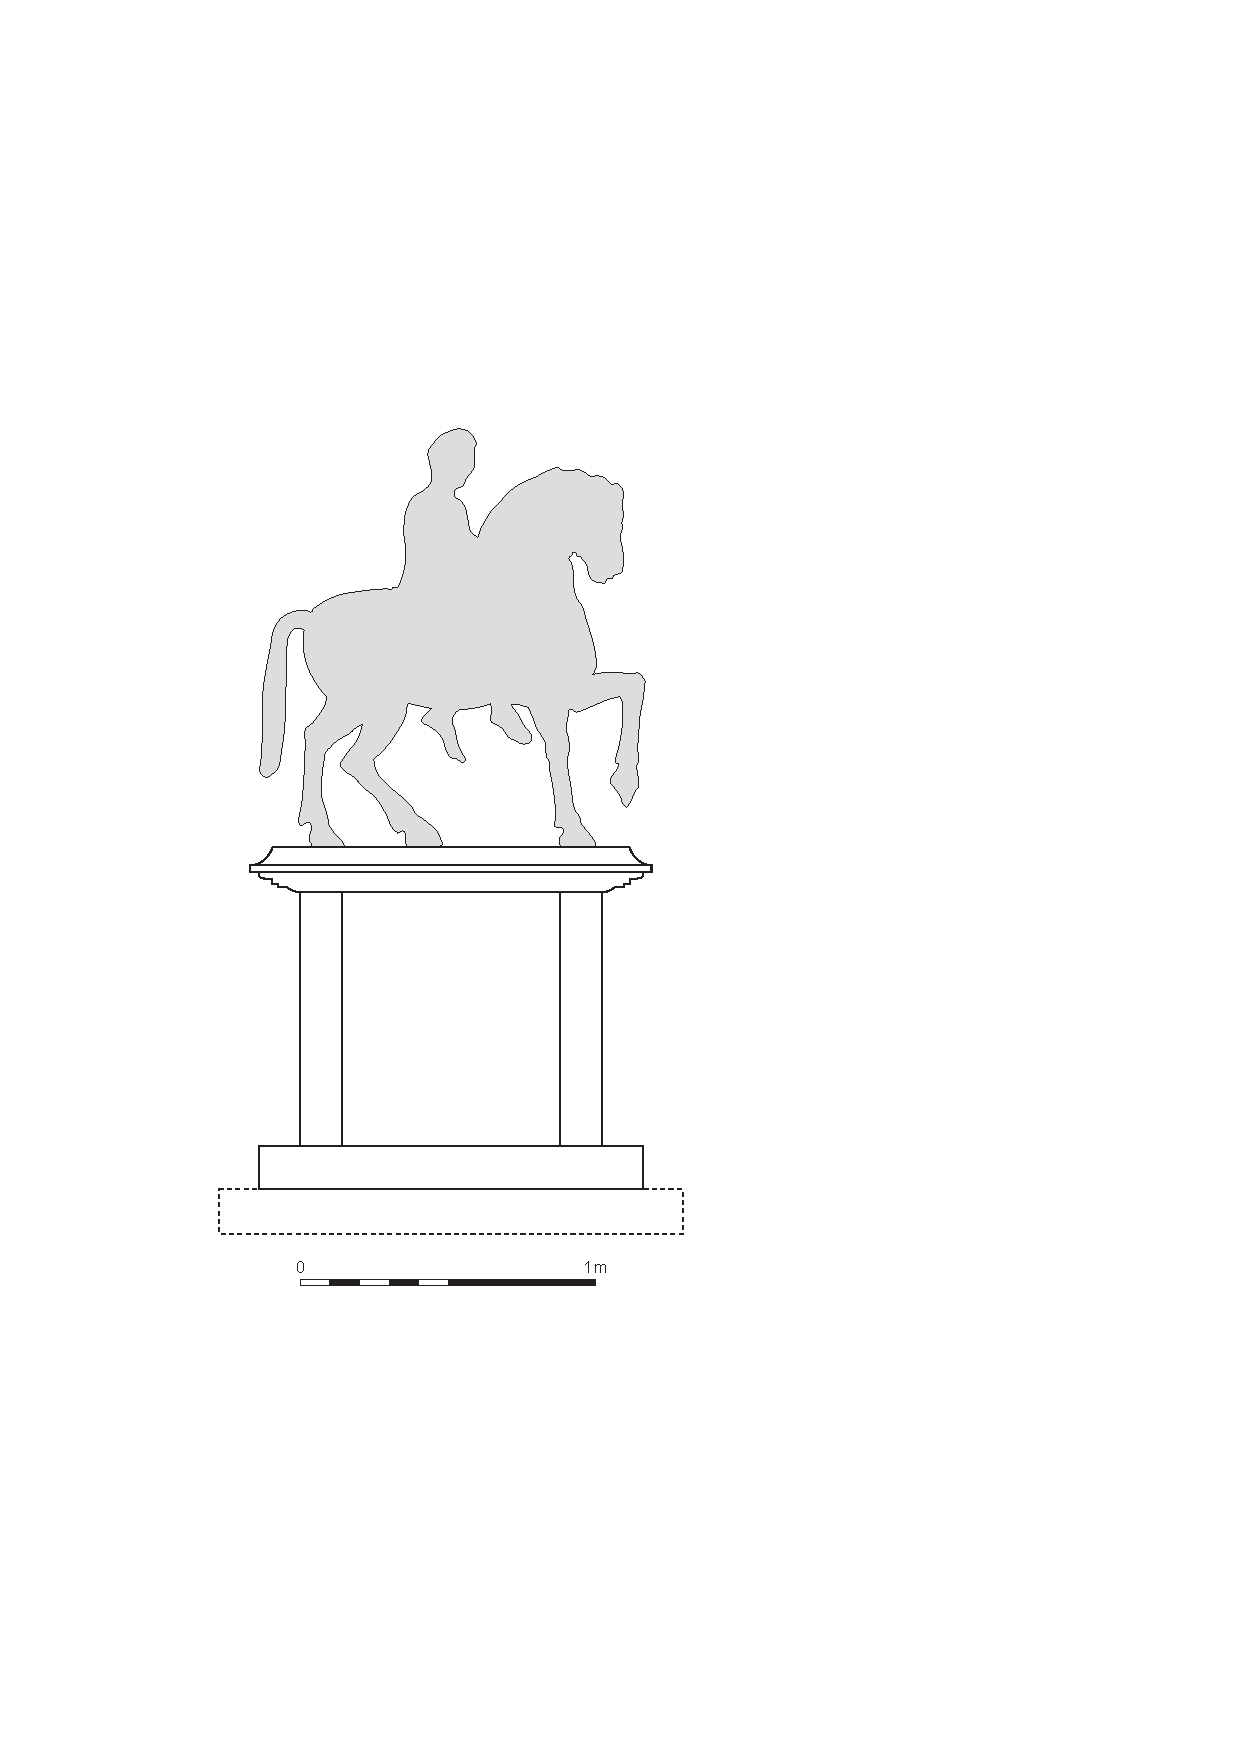
\includegraphics[scale=0.5]{images/fig02ReiterstatueVonDerSeite.pdf}
\caption{Equestrian statue: view from the side}
\label{fig:2}
\end{figure}

Equestrian statues are, nevertheless, not uniform. They can also provide, in turn, 
additional information by their specific appearance. They were dedicated in very 
different forms; above all in very varied sizes. For example: Alfius Secundus, 
a \textit{flamen perpetuus }in Africa proconsularis, set up two or three equestrian 
statues of the emperor Septimius Severus\footnote{\emph{CIL VIII} 14370 (Avedda).}. Even though these statues represent the 
emperor, they must have been small ones because the base is only 54 cm high and 
35 cm wide\footnote{Bergemann (n. \ref{note:18}) no. 81.}. These small equestrian statues fitted probably into the context in which they stood. On the other hand, gigantic equestrian statues were erected of 
all the emperors – and not only of them. An exact relation between the size of 
a monument and social rank did not exist. Various factors could be relevant in 
such cases. Nonetheless, the size can already tell us something about the status 
of the honorand and the intention of the dedicator. 

\begin{figure}[!bp]
\centering
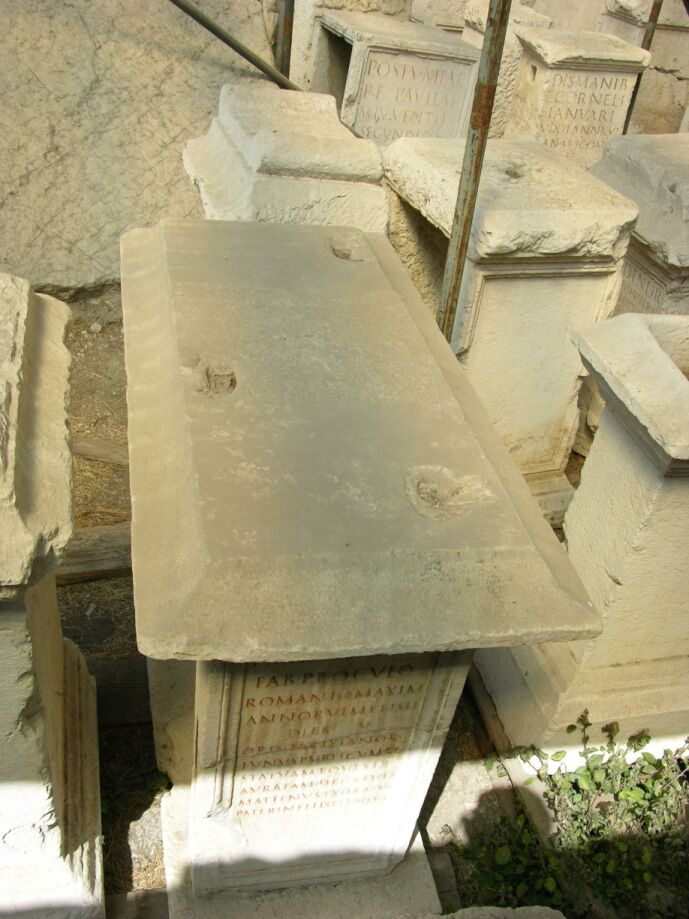
\includegraphics[scale=0.5]{images/fig03}
\caption{Brescia Basis with 2 pillars}
\label{fig:3}
\end{figure}

Most \textit{statuae equestres }either rose from bricked bases or the base was 
made of solid stone. The base for the statue of C. Minicius Italus in Aquileia 
was built with bricks and then covered with marble slabs\footnote{\emph{CIL V} 875 = Dessau 1374 = Inscr. Aquileiae I 495; G. Alföldy, Römische Statuen in Venetia et Histria, Heidelberg 1984, 98 f. no. 87. For a photo see EDCS-01600153.}. The one of the young 
senator L. Fabius Severus in Tergeste was made of a single solid stone\footnote{\emph{CIL V} 532 = Dessau 6680 = Inscr. Italiae X 31. Photo : EDCS-04200621.}. The latter 
applies to the majority of these monuments. Even so, at least in the first century 
AD there was also a type of an equestrian statue that remained unattended in research 
until recently. For there existed equestrian statues, which seemed much lighter 
and did not stand on an apparently solid basis\footnote{\label{fn:30}For the following discussion see W. Eck - H. von Hesberg Tische als Statuenträger, MDAI (R) 111, 2004 [2006], 143 ff.}. Sometimes the base was simply made 
of a foundation slab, two supporting pillars and a cover plate on top, on which 
the equestrian statue stood (Fig. \ref{fig:1} and \ref{fig:2}). To the best of my knowledge, there 
is only one fully surviving example of this type, which is today kept in the museum 
of Brescia. (Fig. \ref{fig:3}) This example presents a posthumous honour for a 6-year old 
boy decreed by the \textit{ordo} \textit{decurionum }of Brixia. The setting up 
of the equestrian statue was executed by the father of the deceased\footnote{\emph{CIL V} 4441 = Inscr. Italiae X 5, 232.}. In this case, 
we recognise such a particular type of equestrian statue only because the entire 
monument survives, in the inscription the father mentioned only a \textit{statua 
equestris}. Yet research did not consider the piece which can be seen in the museum 
at Brescia as a special type of honorary monument, but rather as a unique object. 
There are, however, not a few inscriptions that were connected with this statue 
type in the Roman age. The central feature of this type are always two supporting 
pillars and a cover plate on top, on which the equestrian statue stood. Two kinds 
of pillars can be distinguished, and they differ clearly. There are pillars such 
as those used as inscribed support in the form of the example from Brescia and 
there are the so-called \textit{trapezophora }on which an inscription is not rarely 
found\footnote{For more information see Eck - von Hesberg (n. \ref{fn:30}).}. Just to mention some: we know for the young senator P. Numicius Pica Caesianus\footnote{\emph{CIL VI} 3835 = D 911= VI 31742 = 31743.} 
two \textit{trapezophora }from Rome, quite a number from Torino for Q. Glitius 
Atilius Agricola\footnote{\emph{CIL V} 6974 – 6987; Eck - von Hesberg (n. \ref{fn:30}) 186 f.}, a single one for T. Flavius Cimber, a municipal magistrate from 
Urvinum Mautaurense\footnote{\emph{CIL XI} 6062: \emph{T(ito) Flavio L(uci) f(ilio) Ste(llatina) Cimbro pont(ifici), aed(ili) bis, IIIIvir(o) i(ure) d(icundo), quinq(uennali), praef(ecto) fabr(um), d(ecreto) d(ecurionum)}.} and many others\footnote{See Eck - von Hesberg (n. \ref{fn:30}) 180 ff.: a list of the inscribed trapezophora which were known to us in 2003/4.}.

These epigraphic monuments can partly be found in the EAGLE database too. Here 
one has to search for the term \textit{trapezophorus }as object type\footnote{\emph{Trapezophoron} is the normal \emph{terminus technicus}.}. Table feet 
of this kind, which contain inscriptions, are known in relatively big numbers because 
of their special shape; they have always been categorised individually\footnote{For the literature see Eck - von Hesberg (n. \ref{fn:30}) notes 1-3.}. However, 
they were not hitherto considered as parts of statue bases but rather of tables, 
real \textit{mensae}. Today it is no longer questionable that these \textit{trapezophora 
}with inscriptions were in reality parts of statue dedications, with an equestrian 
statue which stood on this specially arranged base\footnote{Eck - von Hesberg (n. \ref{fn:30}) with the general discussion of this type of honorary monuments.}. As long as these inscriptions 
are marked up with the keyword \textit{trapezophorus }(sic!) in the EAGLE database, 
they can be found without problems. In the Heidelberg database, however, with the 
keyword \textit{trapezophorus/um} one will find nothing, although there are three 
such objects in the database; but there they are\textit{ }registered under the 
keyword \textit{mensa}. If one is entering \textit{mensa }in the EDH, numerous 
and extremely varied objects appear, which have by no means the same function\footnote{For an example of a mensa in the concrete sense: IRT 590: \emph{Ti(berius) Cl(audius) Amicus M(arcus) Heliodorius Apollonides aed(iles) mensas p(ecunia) s(ua) d(ono) d(ederunt)}; the inscription is engraved on the frame of the table; cf. also \emph{CIL III} 15184, 18 = AIJ 310. On the other side also a mensa ponderaria can be found by surging for a mensa: AE 1905, 37 = HD030144; \emph{CIL III} 15025 = HD005744.}. 
If the keyword \textit{mensa }is entered in the EDH and connected with the search 
parameter ``honorific inscription'', it is possible to find three \textit{trapezophora} 
– in the category \textit{mensa}\footnote{HD002671 = EDR111713; HD006112 (Ruck) = EDR076783; HD025725 (Féraudi) = EDR073154 (also described as \emph{mensa}).}. But who would imagine that the combination 
of \textit{mensa} and honorific inscription is necessary to find this type of monument? 
Also in EAGLE not all the objects that belong to this form of monument can be found 
with a single search term. That means as a consequence, that in the databases combined 
by EAGLE the terms for specific objects should be uniform; for the moment this 
is not the case. 

To give one example here: We know one \textit{trapezophoron } with an inscription 
from Cosa in which Drusus Caesar, son of Tiberius, is mentioned; it appears in 
EDR076783 with no specific characteristics for the object, because the information 
comes from the EDH. In EDH006112, the object of this inscription appears as a \textit{mensa} 
and an ``Ehreninschrift'', but not as a trapezophoron. On the other side: In EAGLE, 
\textit{mensa }can almost only be used as long as the word occurs in the inscribed 
text, not as term for an archaeological object\footnote{For an exception see the preceding note.}. Again the harmonization of search 
terms becomes extremely important in order to enable a quick and safe search\footnote{In EDR077116 an inscription with the text: \emph{L(ucius) Ansius Quintill[i]anus m\d{e}[nsam -{}-{}-]} is called trapezophorus, although in reality it is a \emph{mensa}, as the text itself tells us and as the photo in EDCS-10700899 clearly shows. The inscription is engraved on the frame of the tabula for a \emph{mensa}.}.

As mentioned before, a total of 23 \textit{trapezophora}, which can be described 
as honorific monuments for single persons, can be found in EAGLE. These are by 
far not all the inscriptions, which were once connected with equestrian statues, 
which did not stand on a solid base but rather on a plate supported by two pillars. 
The posthumous honours in Brescia for the 6-year old P. Matienus Proculus is, as 
already mentioned, such an example\footnote{\emph{CIL V} 4441 = Inscr. Italiae X 5, 232.}. But in the databases, inscriptions for such 
monuments are not described with their specific features\textbf{ }as\textbf{ }the 
entry for the monument from Brescia makes clear; of course normally they can be 
found with the term honorific inscription, i.e. as \textit{titulus honorarius}; 
but that does not really help, there are too many \textit{tituli honorarii }in 
the database. The text for Publius Matienus Proculus one would not even find with 
the word \textit{titulus honorarius}, because it is categorised as sepulcralis\footnote{EDR090232. The precise terminus would be: \emph{titulus honorarius postumus}.}. 
To single out the different types, one has to describe in the data bases the special 
singularities, which identify the particular functionality of such monuments. Here 
one example.

\begin{figure}[!bp]
\centering
 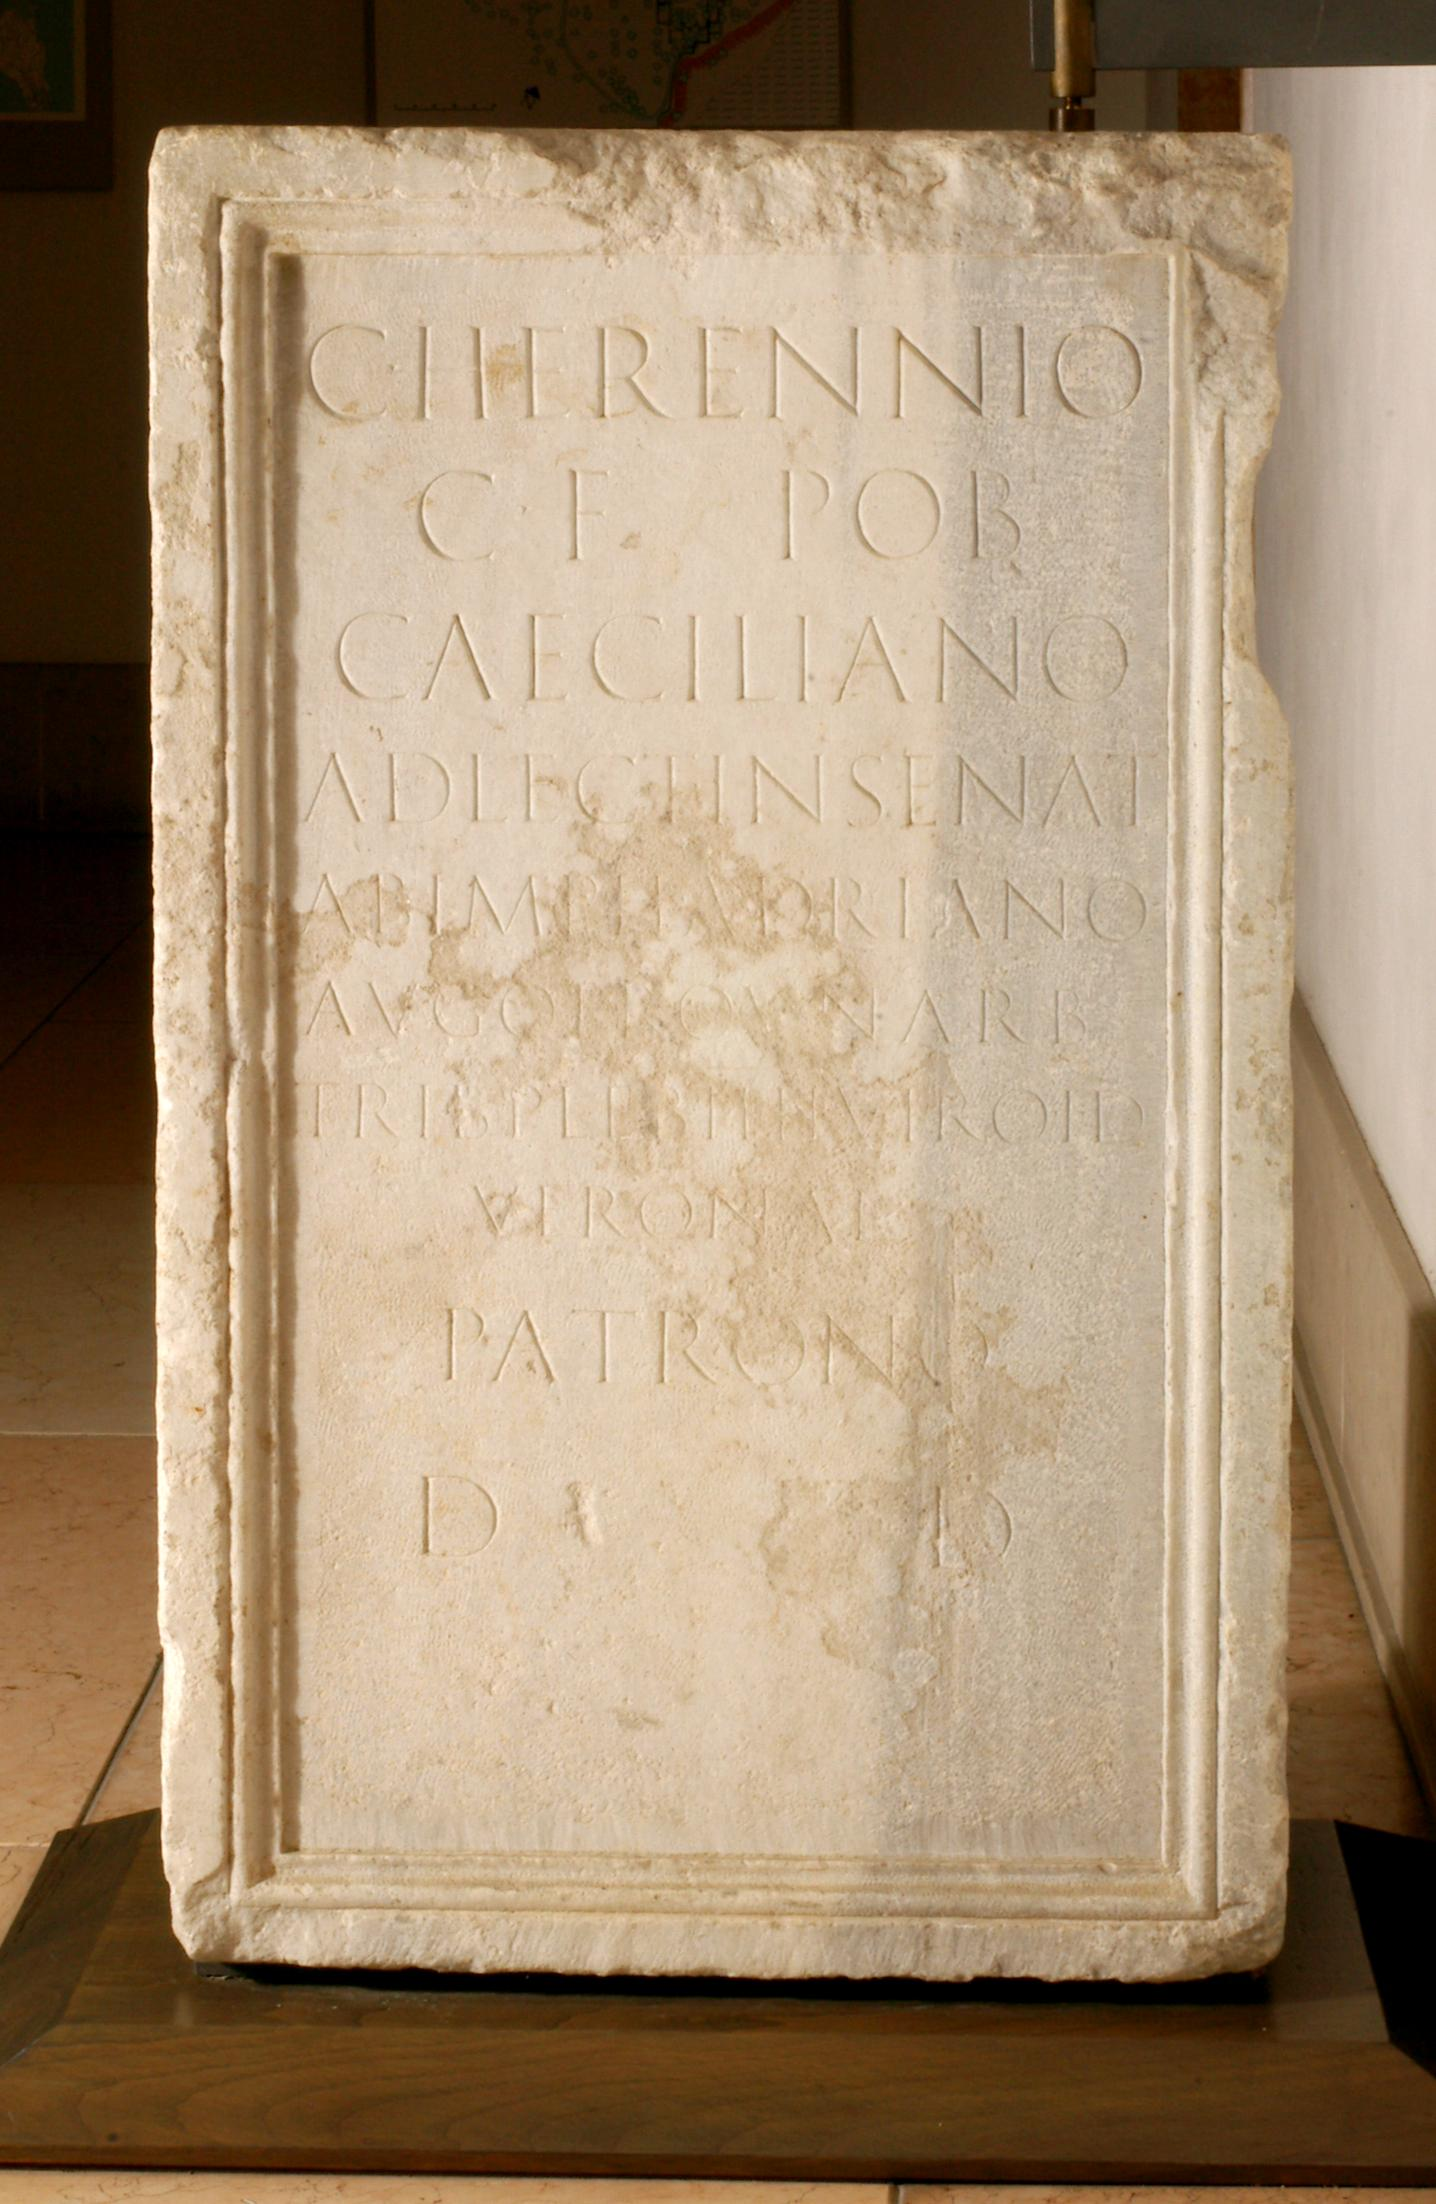
\includegraphics[scale=0.6]{images/fig04}
\caption{Herennius Caecilianus -- frontside}
\label{fig:4}
\end{figure}

In Sirmione (ancient Sirmio), at the Lago di Garda, an inscription was found in 
1960. It once belonged to an honorific monument for the young senator C. Herennius 
Caecilianus. The following text was published by Alberto Albertini in 1973 (Fig. \ref{fig:4})\footnote{\label{fn:46}A. Albertini, Un patrono di Verona del secondo secolo d.C.: G. Erennio Ceciliano, in: Il territorio Veronese in età romana Verona 1973, 439ff. = Alföldy, Römische Statuen (n. 28) 253; R. Bertolazzi - V. Guidorizzi, Supplementa Italiae 28, nr. 7.}:

\begin{quote}
\textit{C(aio) Herennio} \\
\textit{C(ai) f(ilio) Pob(lilia)} \\
\textit{Caeciliano,} \\
\textit{adlect(o) in senat(um)} \\
\textit{ab imp(eratore) Hadriano} \\
\textit{Aug(usto), q(uaestori) prov(inciae) Narb(onensis),} \\
\textit{trib(uno) pleb(is), $\overline{IIII}$viro i(ure) d(icundo)} \\
\textit{Veronae,} \\
\textit{patrono} \\
\textit{d(ecreto) d(ecurionum)}. \\
\end{quote}


The text is not particularly interesting with regard to its content. It only records 
the beginning of a senatorial career in the Hadrianic period. The young senator 
came apparently from Verona where he was also \textit{IIIIvir iure dicundo }and 
patron of the city. For this very reason the city wanted to honour him, naturally 
with a statue. This was also assumed by Albertini, who suggested a bronze statue. 
The text also appears in the EDR and EDH\footnote{EDR093835 and HD033596.}.  



\begin{figure}[!bp]
\centering
 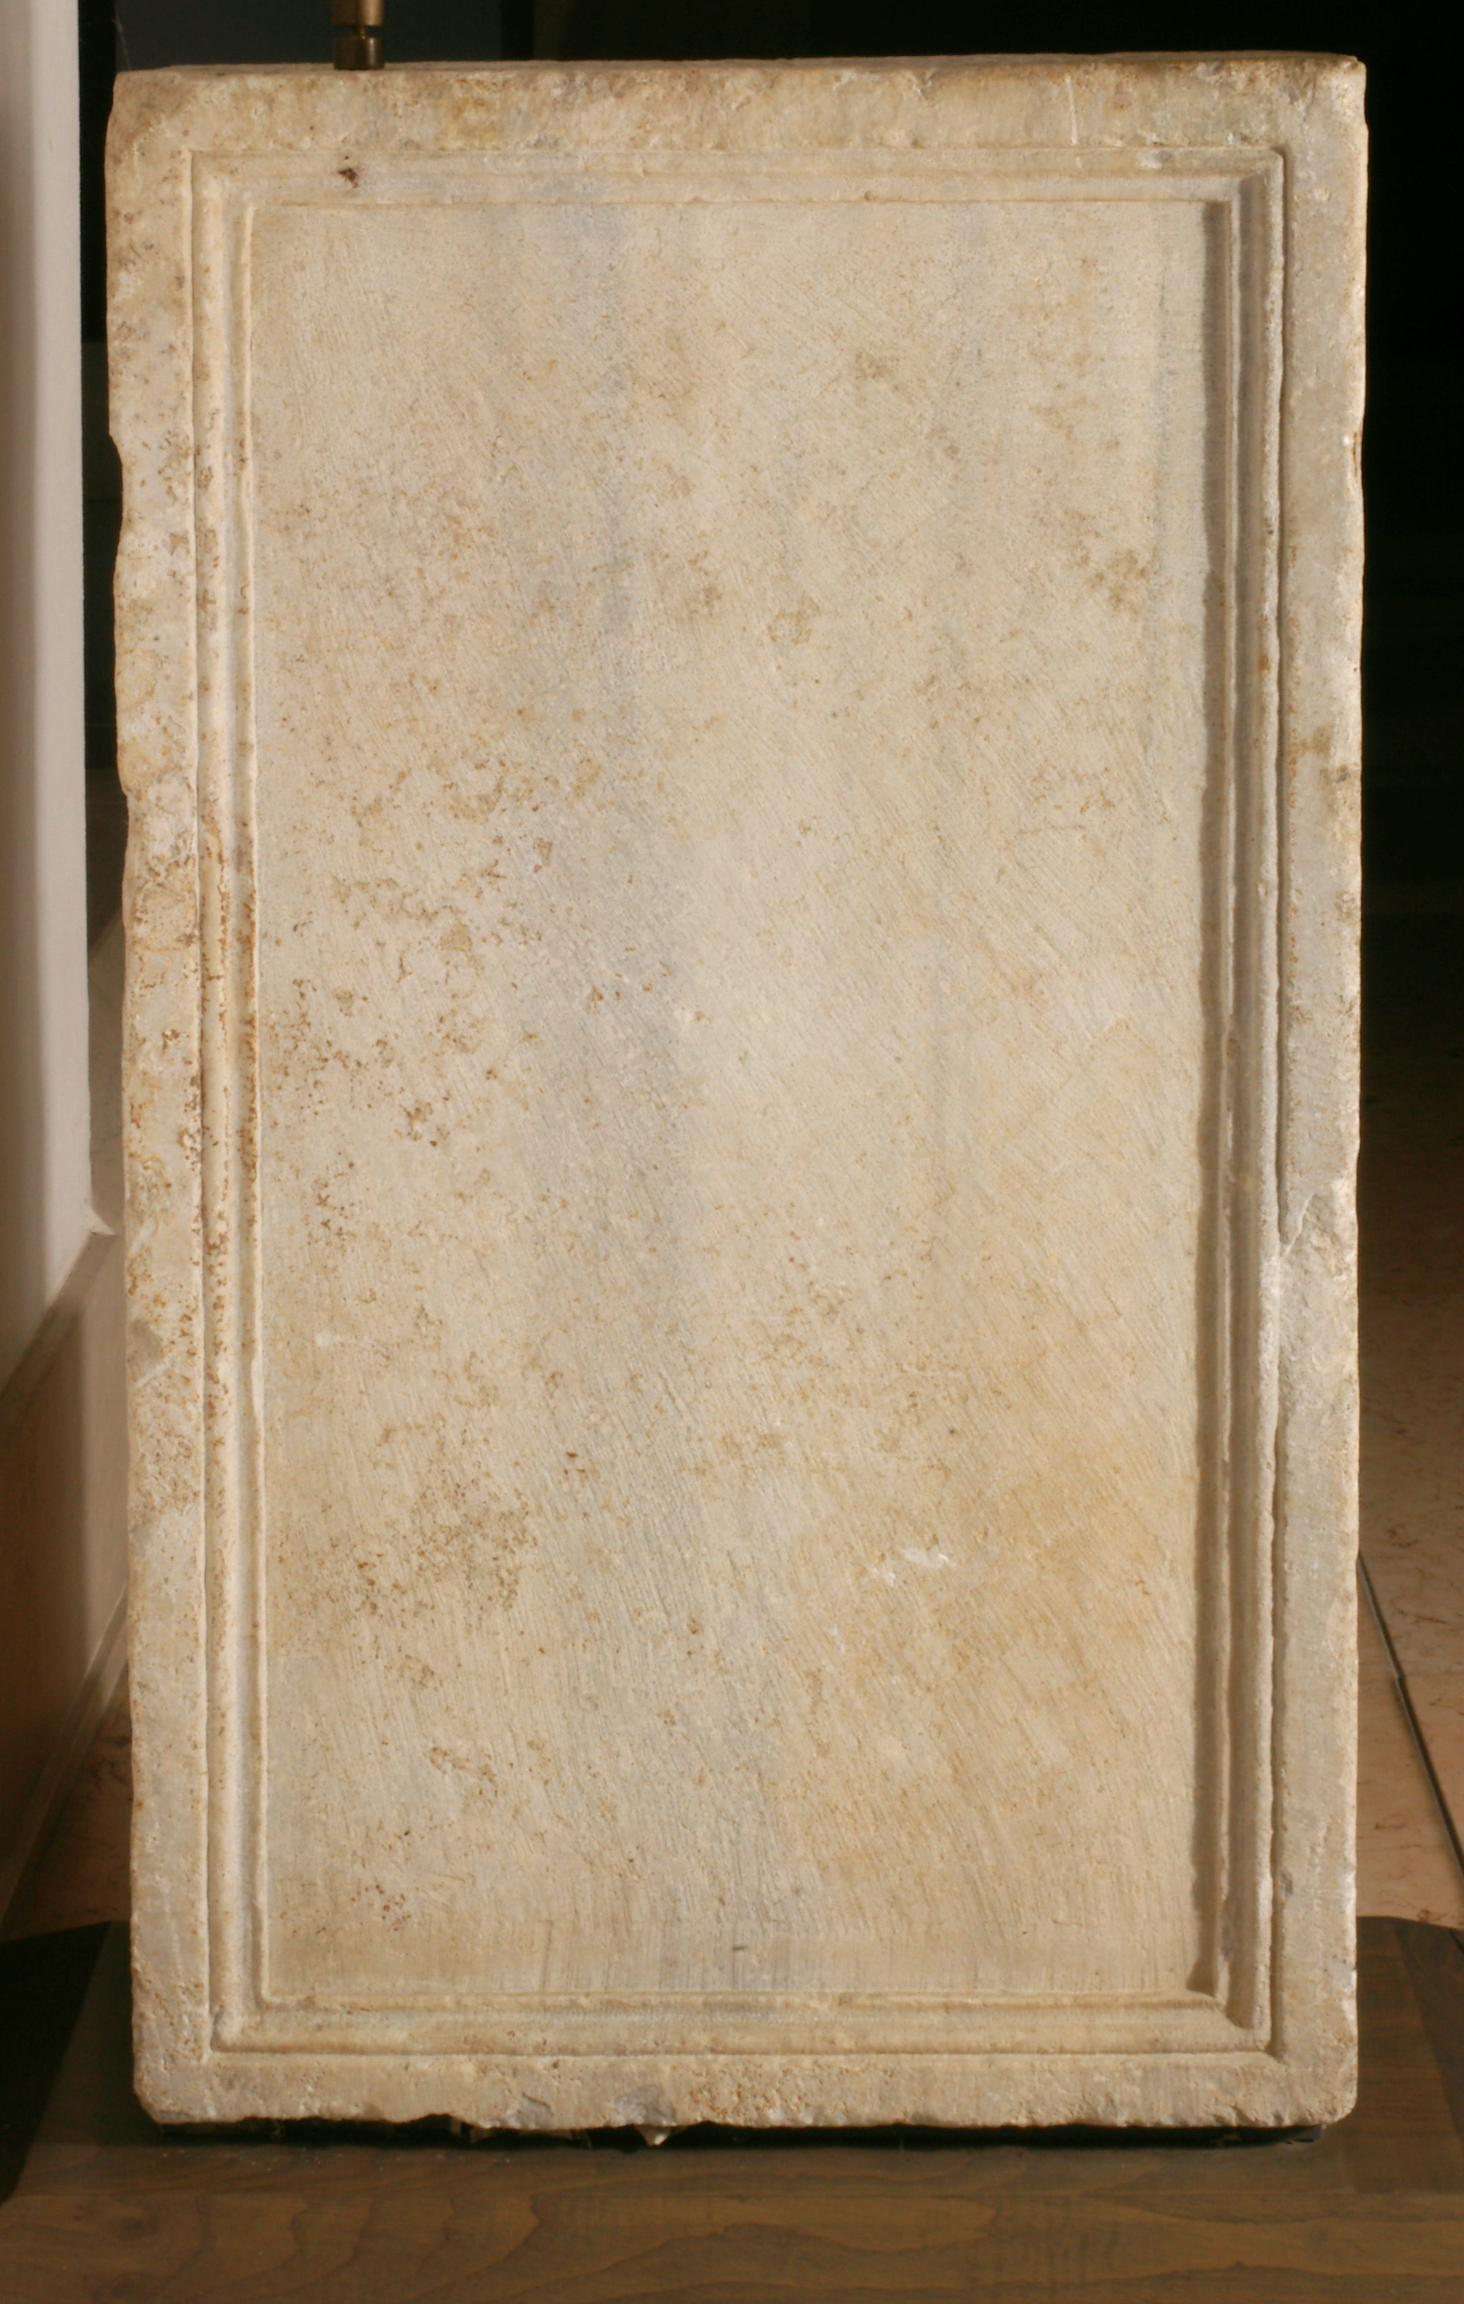
\includegraphics[scale=0.5]{images/fig05}
\caption{Herennius Caecilianus -- backside}
\label{fig:5}
\end{figure}

\begin{figure}[!bp]
\centering
 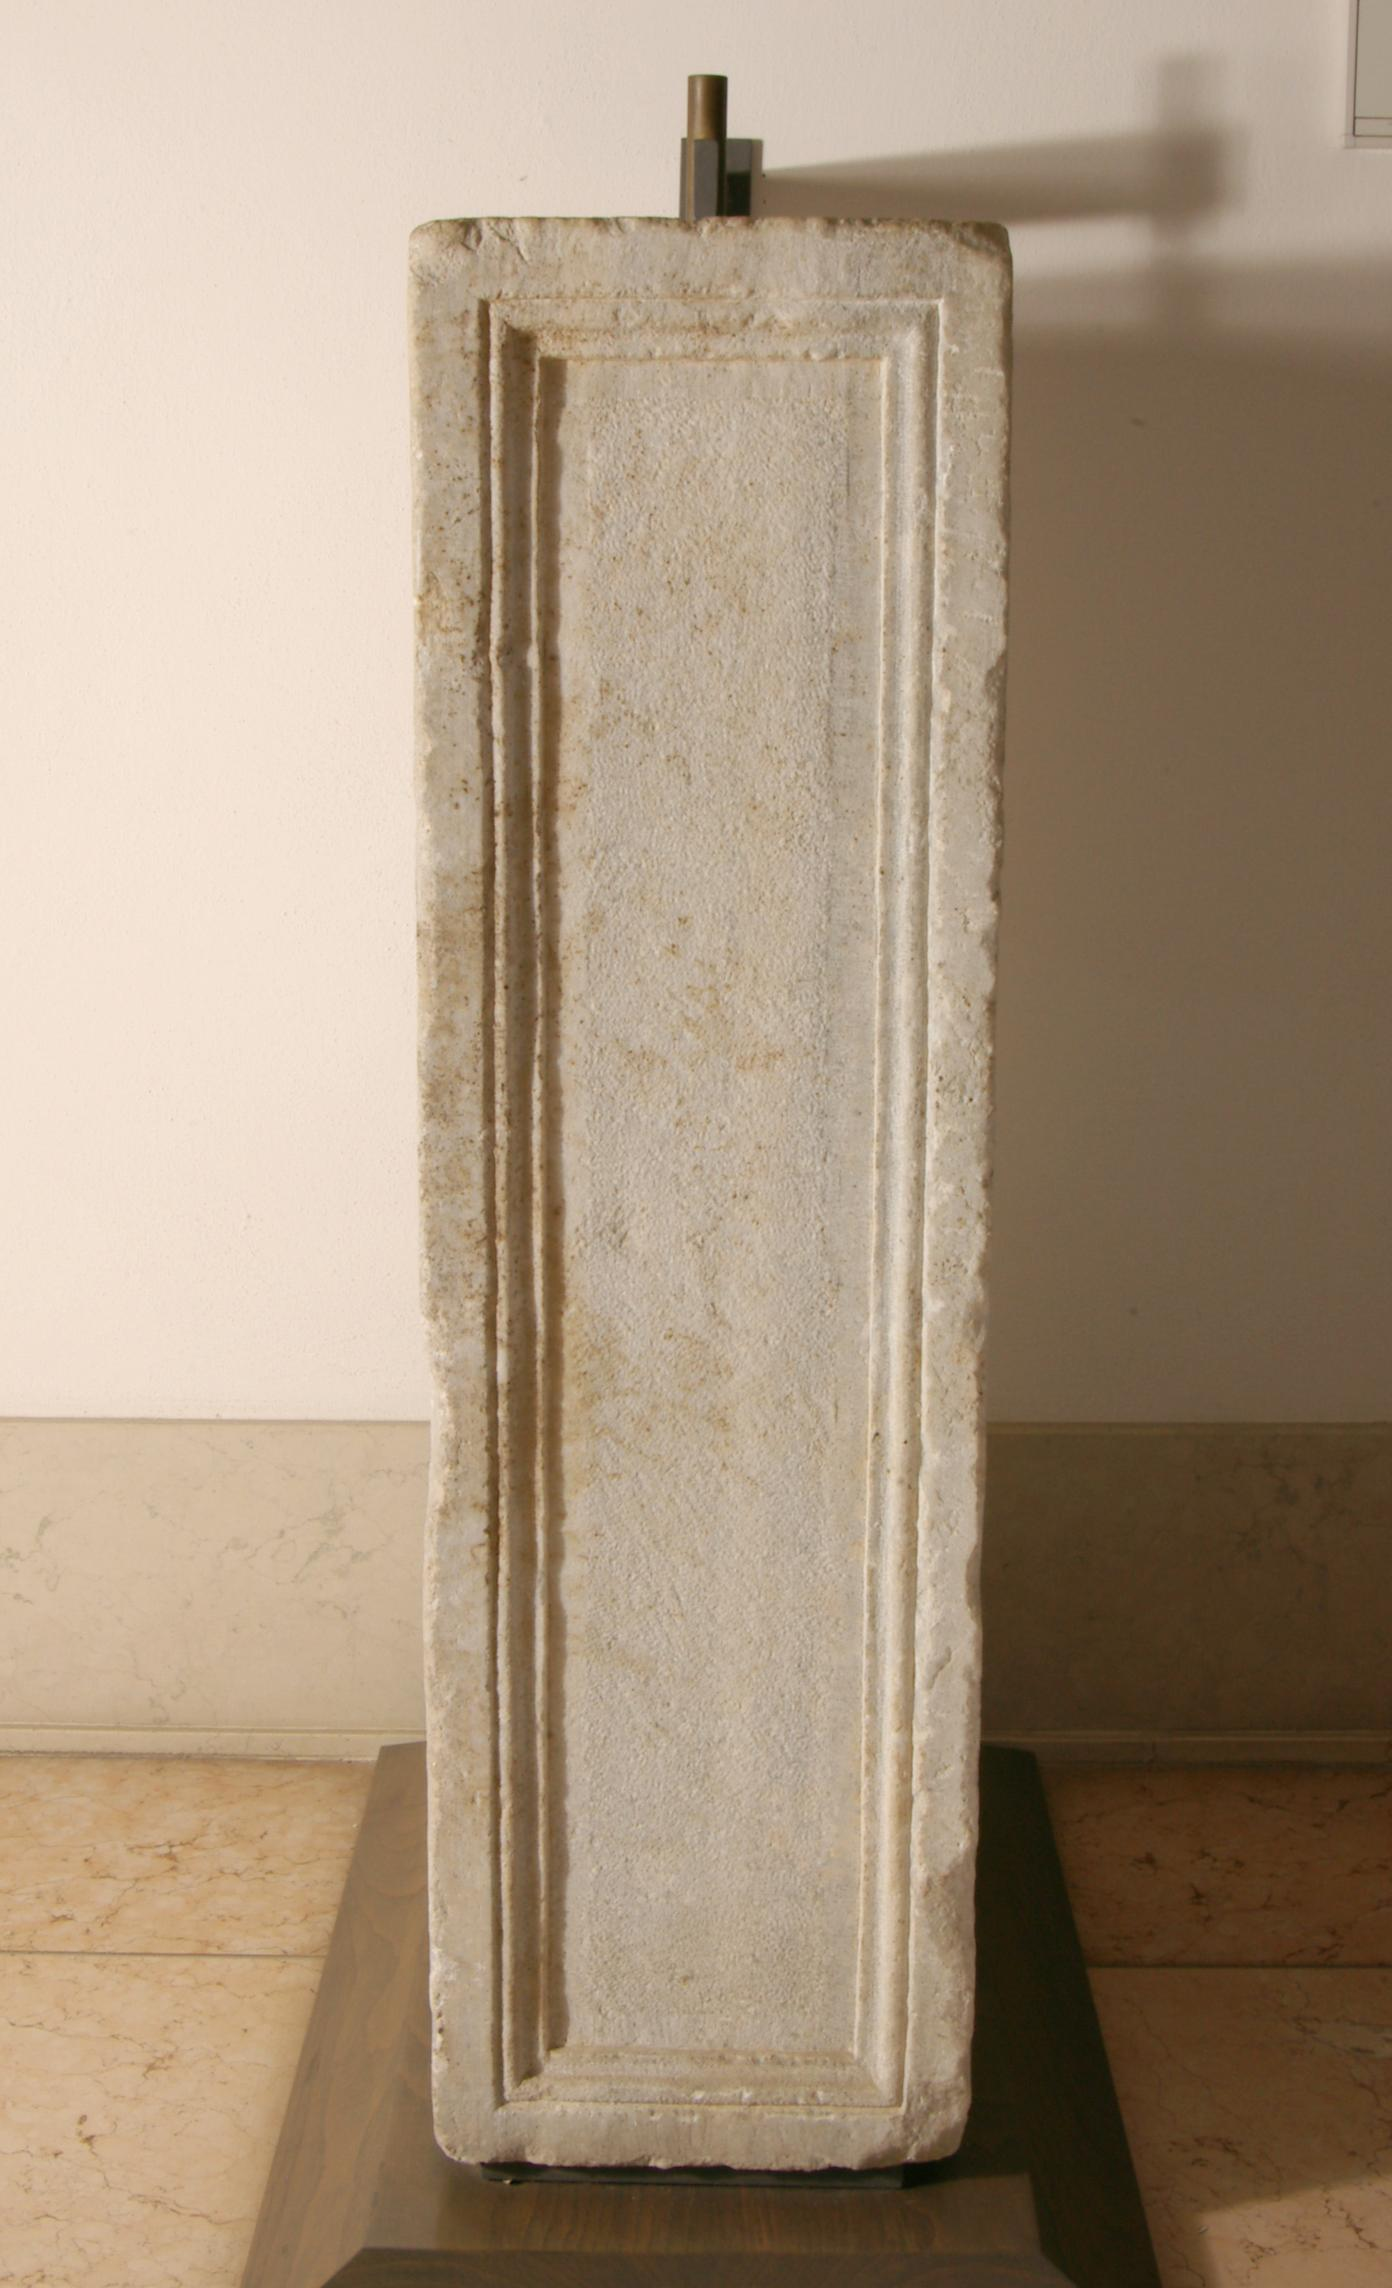
\includegraphics[scale=0.6]{images/fig06}
\caption{Herennius Caecilianus -- lateral}
\label{fig:6}
\end{figure}

\begin{figure}[!bp]
\centering
 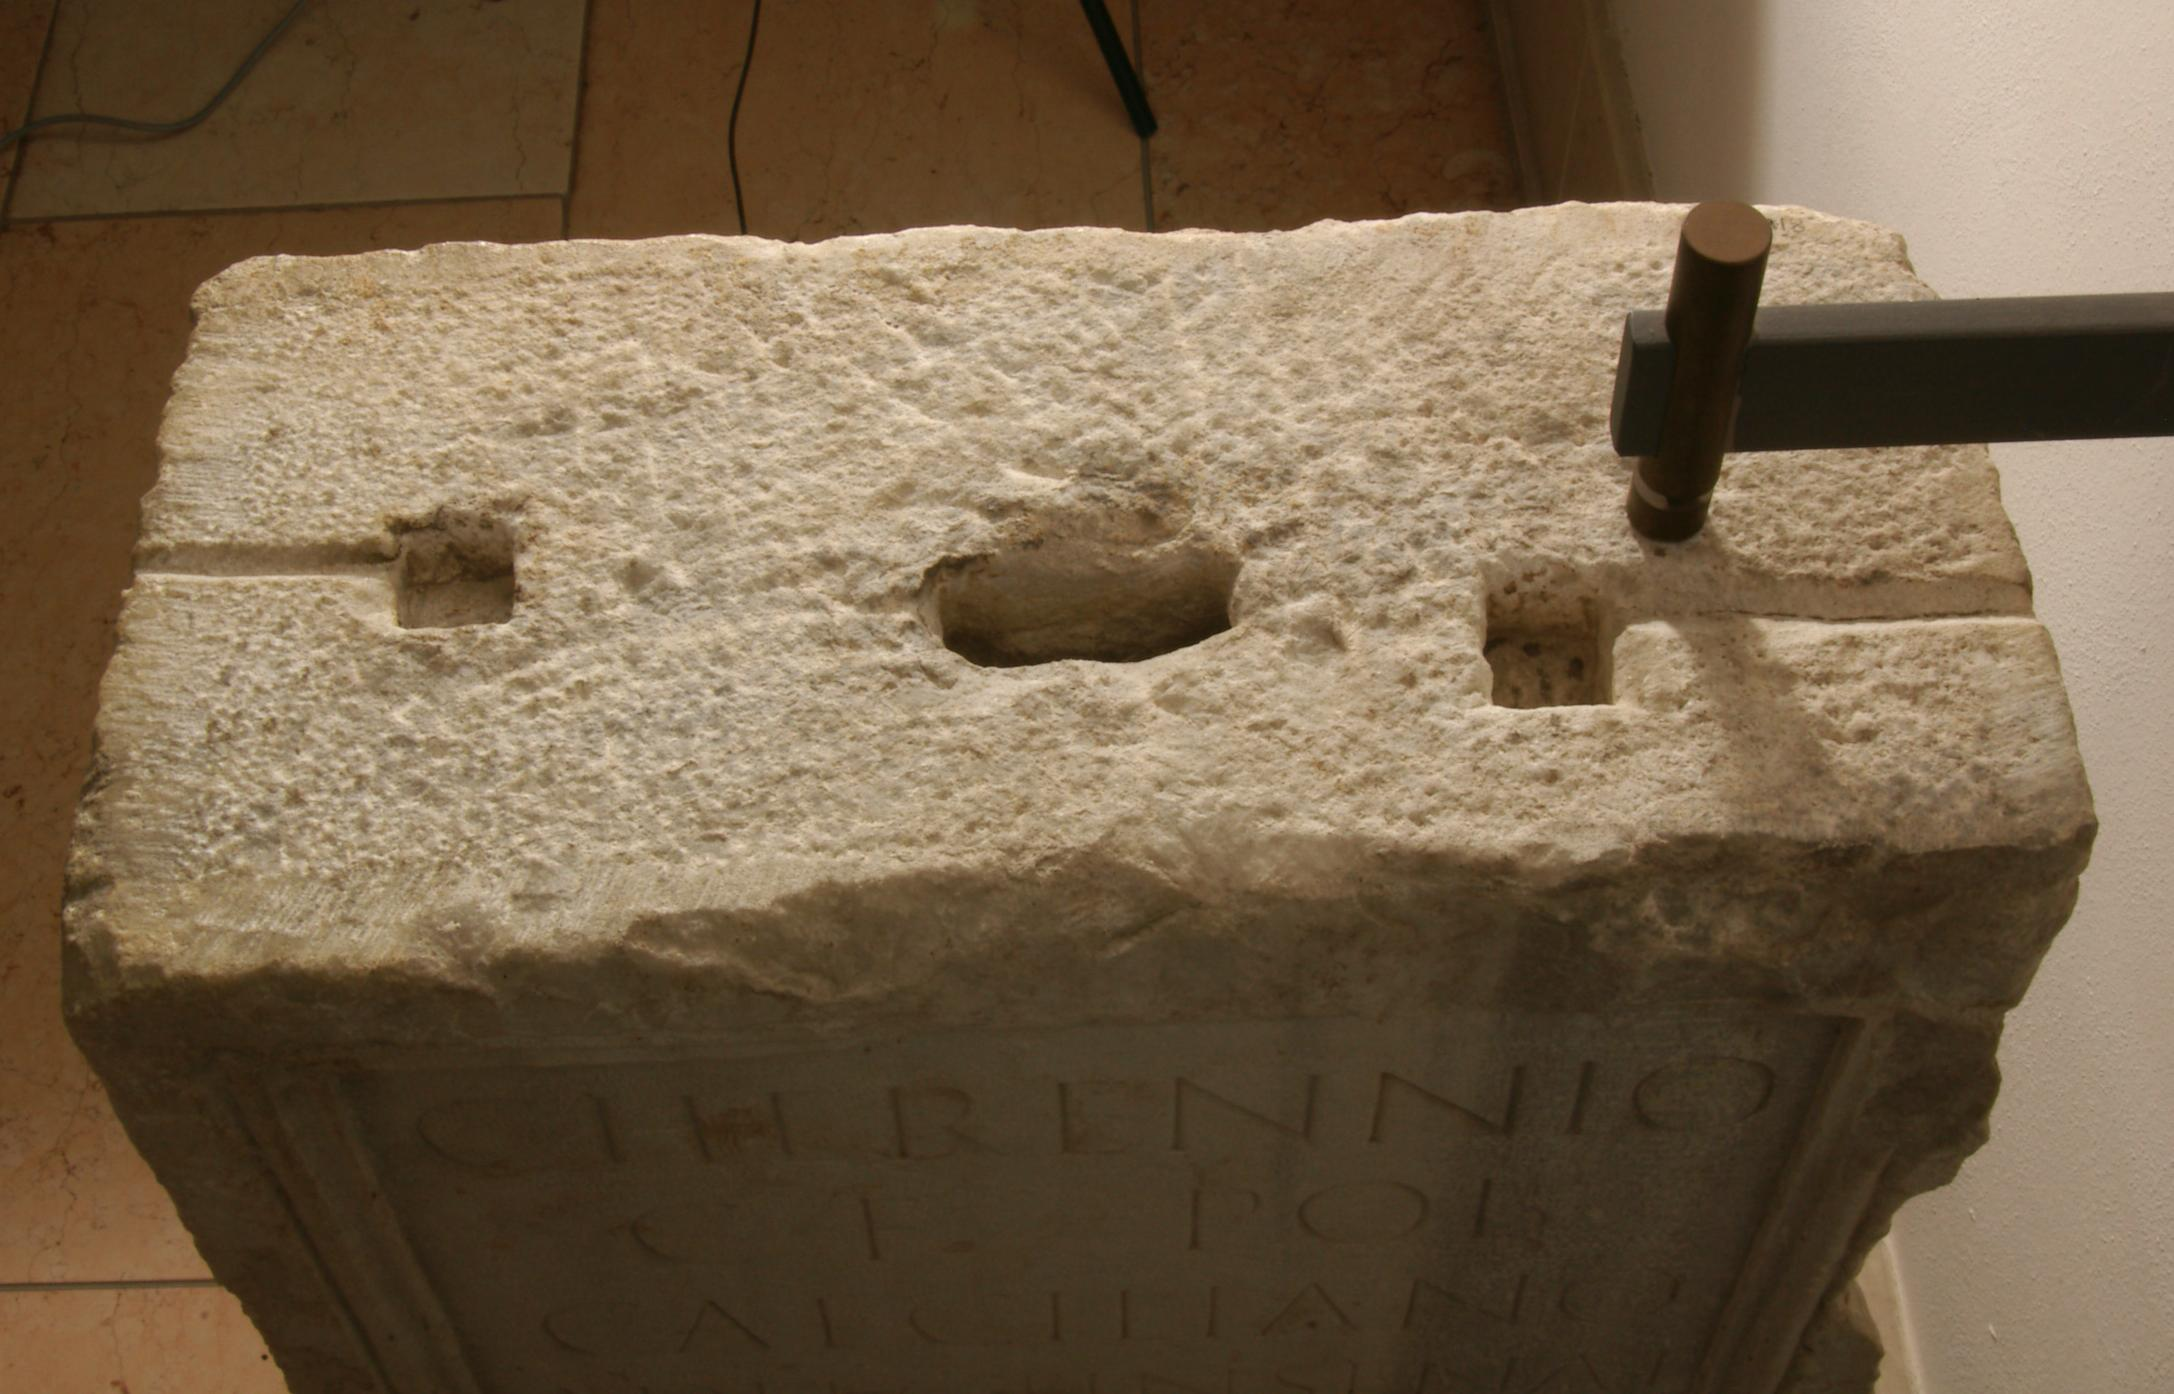
\includegraphics[scale=0.46]{images/fig07}
\caption{Herennius Caecilianus -- from above}
\label{fig:7}
\end{figure}

The inscribed support consists of a slab, 100 cm high, 59 cm wide and 29 cm deep. 
The text is surrounded with a frame on the front side. The same frame surrounds 
also both laterals and, above all, the backside, which is crucial (Fig. \ref{fig:5} and \ref{fig:6}). 
For this shows that the backside was elaborated with the intention to be exposed, 
a detail also observed by Albertini as he accordingly commented that the base (with 
the statue directly standing on it, in his view) was not \textit{adossata a una 
parete, ma eretta in uno spazzio}\footnote{Albertini (n. \ref{fn:46}).}. It is correct that the inscription could not 
have been \textit{adossata a una parete}. However, both the first editor and all 
the others who dealt with the inscription thereafter have simply not wondered how, 
then, could the statue stand on a slab which is only 29 cm deep (Fig. \ref{fig:7}). Furthermore, 
the three holes for the corresponding dowel on the top side of the slab show that 
no statue was fixed there, but rather, something completely different, another 
horizontal slab. If one compares the evidence concerning this inscribed support 
with the equestrian statue of Matienus Proculus in the Museum of Brescia, shown 
before, which also had the backside of the front pillar elaborated with the intention 
to be seen from both sides like also the second uninscribed pillar – the following 
result becomes immediately clear: Herennius Caecilianus was not simply honoured 
with a statue by the people of Verona, but with an equestrian monument standing 
on an cover plate, which was resting on two pillars, whose front side with the 
inscription was 29 cm deep (the second pillar is lost). This ``lighter'' 
version of an equestrian statue was perhaps chosen by Verona because the monument 
should probably be set up in the estate of the senator. The fact that this type 
of monuments was not unusual in this region is shown not only by the posthumous 
monument of Matienus Proculus in the Museum of Brescia, but also by two other pillars 
in the same museum, which are very similar to the monument of Herennius Caecilianus; 
these too are elaborated on the backside with the intention to be exposed. One 
of the pillars bore once an inscription that was later erased\footnote{A more detailed argumentation in Eck, Wie ehrt man Mitglieder der staatlich-städtischen Elite? (n. \ref{fn:12})}, which makes it impossible 
to know who was honoured in such a way (Fig. \ref{fig:8}, \ref{fig:9}, \ref{fig:10}).  

\begin{figure}[!bp]
\centering
 \includegraphics[scale=0.15]{images/fig08}
\caption{Brescia -- erased inscription on a pillar}
\label{fig:8}
\end{figure}

\begin{figure}[!bp]
\centering
 \includegraphics[scale=0.15]{images/fig09}
\caption{Brescia -- pillar}
\label{fig:9}
\end{figure}

\begin{figure}[!bp]
\centering
 \includegraphics[scale=0.05]{images/fig10}
\caption{Brescia -- pillar, reused later}
\label{fig:10}
\end{figure}

What are the consequences of these observations? Databases are by now indispensable 
in the epigraphic work. They speed up not only the work but allow, above all, to 
recognise evolutions through the possibility of examining texts systematically: 
e.g. formulae or forms of abbreviations. Previously, this was only possible through 
the arduous and time-consuming examination of endless volumes. Therefore very often 
this systematic search was not be done or the result was supported only by a slim 
documentary basis. This is now much easier especially when it is possible – like 
now in EAGLE – to access many databases at the same time. In order to achieve 
an even more effective and extensive access, it appears to me, that a stricter 
coordination between the different databases is necessary, a harmonization that 
should also concern the question, which search terms are necessary and possible. 
If the same phenomena, i.e. inscriptions, which had the same function, are shown 
with different terms, a uniform search becomes necessarily difficult, if not completely 
impossible. I referred to the already examined terms \textit{trapezophoron} and 
\textit{mensa}. Under the same term, phenomena and documents with very different 
functions should not appear together. A \textit{mensa }should not refer both to 
a \textit{mensa ponderaria} and, at the same time, to the pillars of an equestrian 
statue of the type described above, as somehow occurred in Cosa with the \textit{trapezophoron 
}for Drusus Caesar. 

The honours for Herennius Caecilianus introduce another further possibility to 
make the utilization of databases for the users even more diverse. In EDR093835, 
a photograph of the monument of Herennius Caecilianus was published, naturally 
of the front face with the inscription. Yet a photograph of the backside would 
be equally necessary to recognise the specific function of the stone and to make 
it immediately clear that the slab was elaborated with the intention to be exposed. 
In this way the essential evidence for its function would be provided. Of course 
such photographs are not always available. However, during the preparation of entries 
one should always check whether more pictures are available and not only those 
of the side with the text. The text remains essential, but it must be completed 
with exact observations about the support of the inscription. Often the meaning 
of the monument can only be reached in this way. This was the central theme of 
the 14\textsuperscript{th} Congress of Epigraphy. Databases have the capacity to 
provide all those details which are necessary for the complete interpretation of 
an epigraphic monument\footnote{For the acts of the Congress see n. \ref{fn:7} above.}. The high costs that the inclusion of many pictures in previous 
publications entailed are not a crucial problem any longer. 

\begin{figure}[!bp]
\centering
 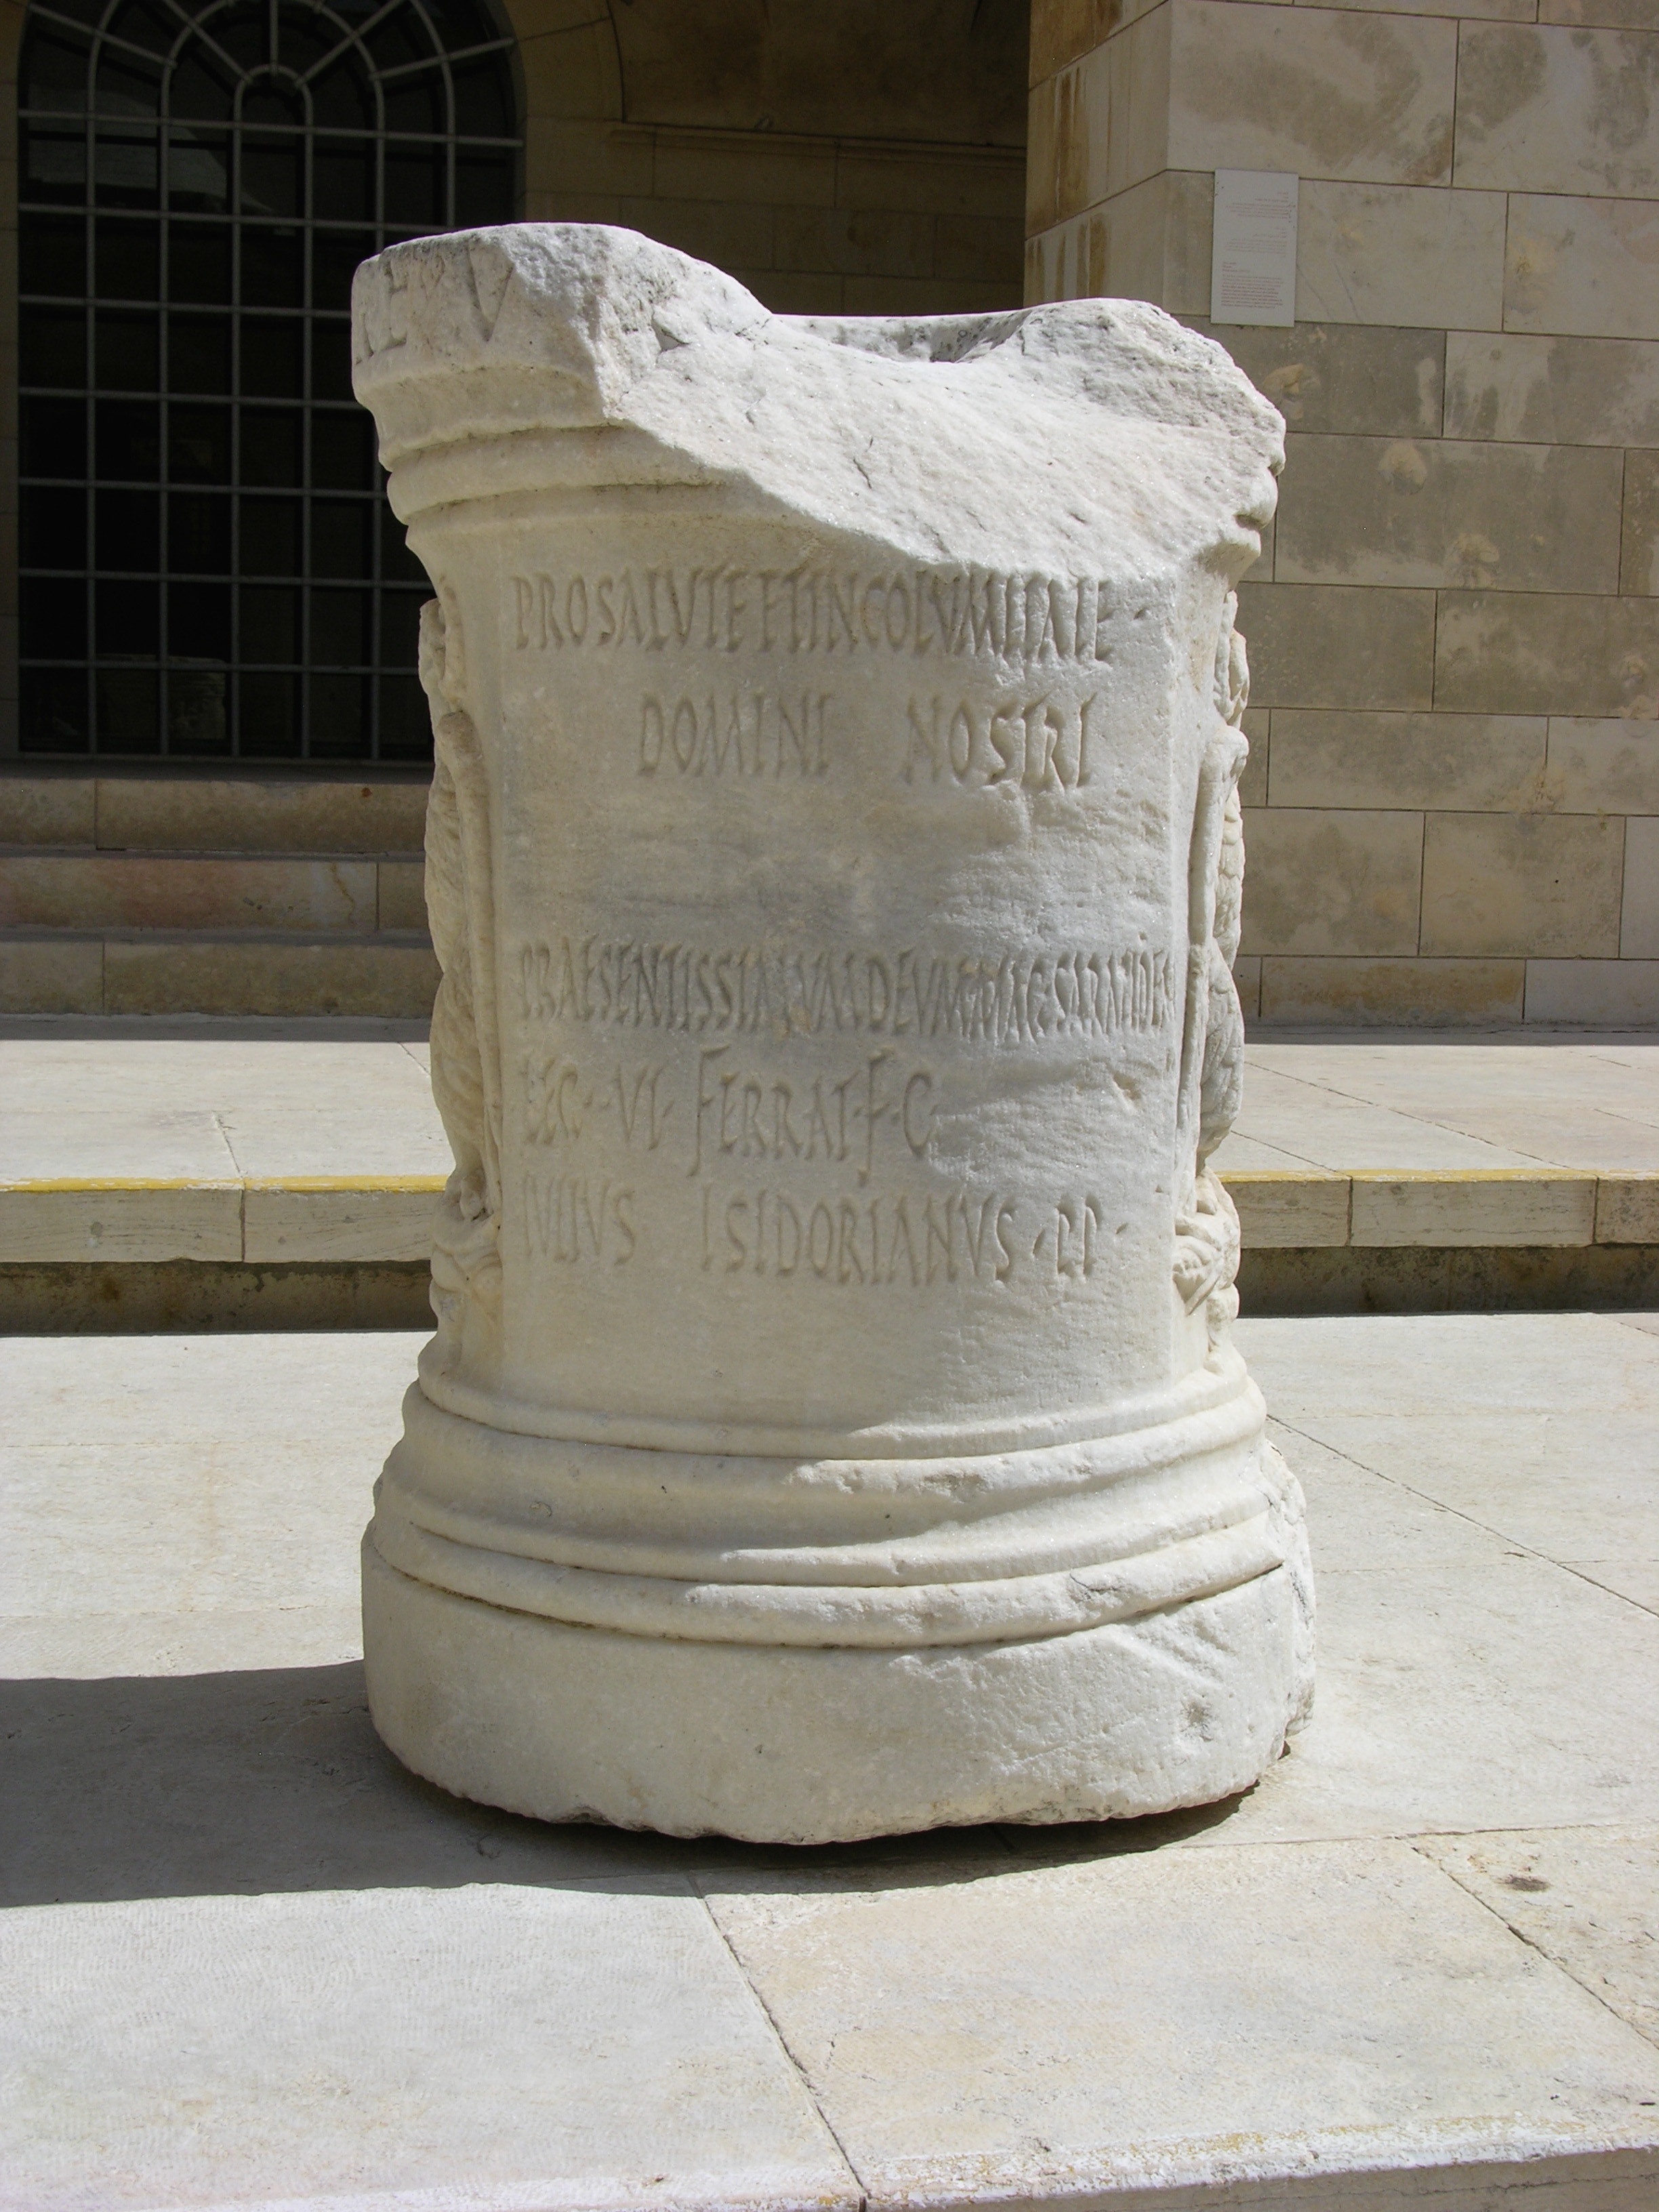
\includegraphics[scale=0.06]{images/fig11}
\caption{Base, Sarapis dedication -- Front}
\label{fig:11}
\end{figure}

\begin{figure}[!bp]
\centering
 \includegraphics[scale=0.06]{images/fig12}
\caption{Base, Sarapis dedication -- Eagle}
\label{fig:12}
\end{figure}

\begin{figure}[!bp]
\centering
 \includegraphics[scale=0.06]{images/fig13}
\caption{Base, Sarapis dedication -- Victoria}
\label{fig:13}
\end{figure}

\begin{figure}[!bp]
\centering
 \includegraphics[scale=0.06]{images/fig14}
\caption{Base, Sarapis dedication -- Eagle}
\label{fig:14}
\end{figure}

At the end of my presentation let me once more demonstrate the necessity to describe 
clearly the monumental features of an inscription and the photographic documentation 
now with an example that comes from the material of the \textit{Corpus Inscriptionum 
Iudaeae/Palaestinae}\footnote{This monument will be included in volume V of the Corpus Inscriptionum Iudaeae/Palaestinae.}. A short time ago one could find the inscription only in the 
database Clauss-Slaby and only the text\footnote{EDCS-15200169; now there are also photos connected to the text. Under the adresse: \url{http://www.antiquities.org.il/t/item_en.aspx?CurrentPageKe y=33&rock=0} the monument can be seen on the homepage of the Rockefellermuseum in Jerusalem; there is only mentioned that an inscription is written on the monument; but the text is not given}. Avi Yonah, who greatly contributed to 
the collection and publication of epigraphic monuments during the time of the British 
mandate in Palestine, published in 1946 an inscription found near the legionary 
camp of the \textit{legio VI Ferrata}, near Caparcotna = Legio\footnote{M. Avi-Yonah, Newly discovered Latin and Greek inscriptions, QDAP 12, 1946, 89 = AE 1948, 145.}. It is a round monument, 
1.05 m high, which he – like many epigraphists later – presented as an altar\footnote{For example. L. Vidman, Sylloge inscriptionum religionis Isiacae et Sarapiacae, Berlin 1969, 182f. no. 361; F. Mora, Prosopographia Isiaca. I. Corpus Prosopographicum Religionis Isiacae, Leiden – New York – Kopenhagen – Köln 1990, 243 Nr. 577; N. Belayche, Iudaea-Palaestina, The Pagan Cults in Roman Palestine (Second to Fourth Century), Tübingen 2001, 59 ff.; L. Bricault, Recueil des inscriptions concernant les cultes isiaques (RICIS), 3 vols., Paris 2005, 508f. no. 403/0201; N. Belayche, Les dévotions à Isis et Sérapis dans la Judée-Palestine romaine, in: Nile into Tiber. Egypt in the Roman World, hg. L. Bricault – M.J. Versluys – P.G.P. Mayboom, Leiden 2007, 451f.; W. Eck, Rom und Judaea. Fünf Vorträge zur römischen Herrschaft in Palaestina, Tübingen 2007, 186f.; P. Figueras, The Pagan Image of Greco-Roman Palestine and Surrounding Lands, Oxford 2013, 78. 96.}. 
The monument shows three perfectly elaborated relieves on three sides: a Victoria 
standing on a globe with a tropaion as well as a victory crown in the hands, and 
two eagles that carry a thunderbolt in the crawls and a crown in the beak. The 
inscription on the front face reads (Fig. \ref{fig:11}, \ref{fig:12}, \ref{fig:13}, \ref{fig:14})\footnote{The text of the inscription is the one corrected by W. Eck, Sarapis und die legio VI Ferrata. Die Weihung einer Sarapisbüste für das Wohl des Kaisers, ZPE 198, 2016 (in print).}:

\begin{quotation}
\textit{Pro salute et incolumitate / domini nostri [[Imp(eratoris) Caes(aris) M(arci) 
Aur(eli) Antonini Aug(usti)]] / praesentissimum deum Mag(num) Sarapidem / leg(io) 
VI Ferrat(a) F(idelis) C(onstans) [[Antoniniana]] / Iulius Isidorianus p(rimus) 
p(ilus).}
\end{quotation}

\begin{figure}[!bp]
\centering
 \includegraphics[scale=0.06]{images/fig15}
\caption{Base, Sarapis dedication -- Upper side}
\label{fig:15}
\end{figure}

In the scholarly discussion, the monument was almost universally presented as an 
altar and logically considered as a dedication \textbf{to} the god Sarapis.\textbf{ 
}Nevertheless, this understanding did not take into consideration the clear testimony 
of the inscription, in which it is written: \textit{praesentissim}\textit{\textbf{um}}\textit{ 
de}\textit{\textbf{um}}\textit{ Mag(num) Sarapid}\textit{\textbf{em}}\footnote{One exception: O. Stoll, Zwischen Integration und Abgrenzung. Die Religion des römischen Heeres im Nahen Osten. Studien zum Verhältnis von Armee und Zivilbevölkerung im römischen Syrien und den Nachbargebieten, St. Katharinen 2001, 280, who saw the consequences of the accusativ for the interpretation of the monument.}. This evidently 
means that Sarapis is not mentioned here as the one to which something was dedicated 
but rather that his figurative representation is the dedicated object. There is 
no doubt that a representation of Sarapis was set up as a votive gift, probably 
in a shrine, perhaps for Egyptian gods near the camp of the legio. The fact that 
a representation of Sarapis was dedicated means, consequently, that we are not 
dealing with an altar but with a base on which the representation found its place. 
Above all, it should not have been omitted from the beginning that there is a remarkable 
peculiarity on the upper side of the base,\textbf{ }namely a completely rounded 
hollow with a diameter of 29 cm and a depth of 9 cm (Fig. \ref{fig:15}). It is an almost 
half sphere that was perfectly chiselled and smoothed from the marble. Sometimes 
earlier scholars noticed this hollow, as already Avi Yonah, but concluded that 
over the ``altar'' a focus would have stood in the hollow, on which the offerings 
could be given. However, a shallow cavity can be seen in such cases at the most, 
but not the half spherical hollow found here. As this half sphere can only be carved 
with a considerable amount of work, it must have a specific meaning, which should 
be connected, as the entire monument, with the depiction of the god Sarapis.   

\begin{figure}[!bp]
\centering
 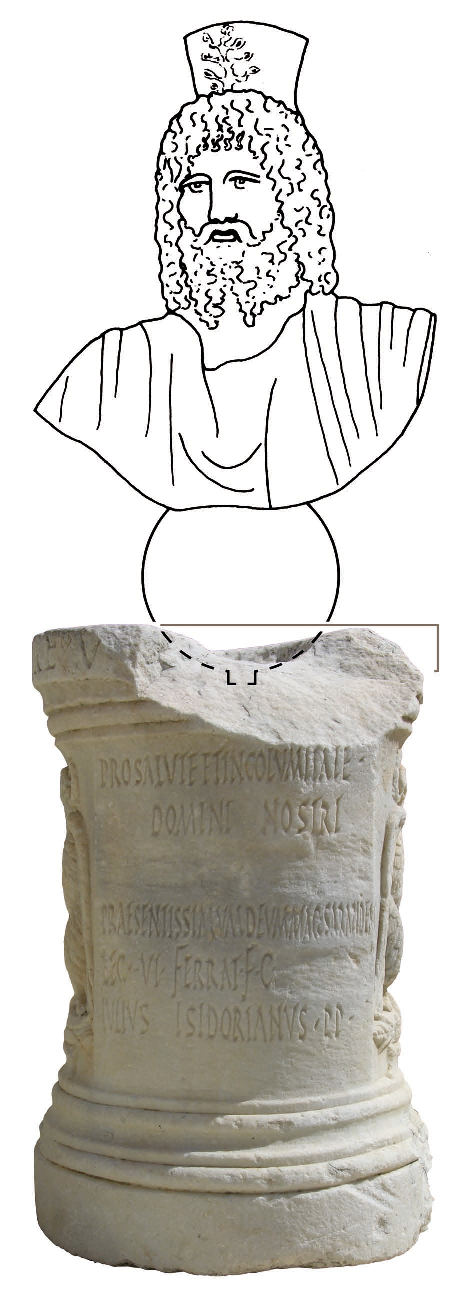
\includegraphics[scale=0.5]{images/fig16}
\caption{Base, Sarapis dedication -- Reconstruction of the bust of Sarapis}
\label{fig:16}
\end{figure} 

The representation of the god is not preserved, only the basis with the inscription 
like in most other dedications. Nevertheless, if one checks the forms 
in which Sarapis is figuratively represented, one immediately comes upon busts 
of the god which sits on a globe. With this observation, we also have immediately 
an explanation for the spherical form of the hollow carved on the upper part of 
the base. Here the lower part of a globe would sink, on which the bust 
of the god would likewise rest. This entire monument, the basis and the bust of 
the god was set up in a shrine and probably took an important place there (Fig. \ref{fig:16})\footnote{Drawing of the reconstruction by Gisela Michel.}. 

As already mentioned, this extra-unusual object appeared until a short time ago 
only as a text in the database Clauss-Slaby. The way in which it should be presented, 
so that users of databases can decipher its complete meaning, follows with necessity 
after the previous discussions: not only must all the sides be depicted but even 
more important is the upper surface for which also the dimensions should be given 
in this case. At least several photos of the monument are now visible in the database 
Clauss-Slaby. Indeed, only all this information together can reveal as much of 
the context as possible. 

These observations in one way or another are valid for all of our epigraphic texts. 
The text alone is not enough, but needs - as far as possible – all the other 
concrete details and photos not only of the text, but of the monument itself. In 
such a way the access to ancient reality becomes easier, as, for example, in the 
villa of Herennius Caecilianus in the area of Sirmione or at the shrine near Caparcotna/Legio 
in northern Galilee. It is clear that we cannot completely reconstruct ancient 
reality, but we should come as close as possible to the former reality. The digital 
presentation is a crucial premise for this purpose. 

\end{document}


